\documentclass[conference]{IEEEtran}
\usepackage[T1]{fontenc}
\usepackage{mathptmx}
\usepackage{amsmath}
\usepackage{graphicx}
\usepackage{booktabs}
\usepackage{balance}
\usepackage{url}
\title{Design and Evaluation of a Two-Way Set-Associative Cache with Exact LRU}
\author{\IEEEauthorblockN{Aaditya Yadav, Gauri Mishra, Bhumi Rastogi, Ansh Sharma, and Anugra}}
\begin{document}
\maketitle
\begin{abstract}
This project implements a blocking, 128-byte cache in Verilog with sixteen
sets, two ways per set, four-byte lines, exact least-recently-used replacement,
and write-back with write allocation. Phase II evaluates the implementation
against an equal-data-capacity direct-mapped baseline using a shared controller
and memory timing model. Eight deterministic workloads execute 2,048 accesses
each on both organizations. An independent software model checks all 32,768
benchmark transactions for hit classification, returned data, refill traffic,
dirty victim addresses, write-back payloads, and latency. All checks pass.
For an alternating pair of conflicting addresses, two-way associativity
reduces misses from 2,048 to two. Wider random and mixed-write traces show
similar or slightly worse latency for the two-way design. These results
demonstrate workload-dependent effects of associativity under a fixed-delay
behavioral memory model.
\end{abstract}
\begin{IEEEkeywords}
cache memory, set associativity, LRU, write-back, Verilog, verification
\end{IEEEkeywords}

\section{Literature Review}
Cache design exploits temporal and spatial locality by retaining a small
working set near a processor. A direct-mapped cache assigns each memory block
to one location, simplifying tag lookup and selection. Set associativity
allows several blocks to share a set and can reduce conflicts, while adding
tag comparisons, selection logic, and replacement state. Hill and Smith study
the relationship between associativity and miss behavior~\cite{hill}. Their
work motivates comparing organizations at equal capacity and evaluating
several address patterns instead of assuming a universal benefit.

LRU evicts the resident block with the oldest most recent reference. Stack
processing, described by Mattson \emph{et al.}, provides a framework for
evaluating storage hierarchies and replacement behavior~\cite{mattson}.
For two ways, exact LRU needs one bit per set. After either way is accessed,
the other way is the next replacement candidate. Wider exact-LRU structures
need more state. Tree-based pseudo-LRU approximates order, FIFO records
insertion order, and random replacement avoids maintaining recency.
Our design uses exact LRU because its two-way implementation is small and
its replacement decisions are straightforward to verify.

Write-back postpones memory updates until dirty-line eviction and therefore
requires a dirty bit and a correct victim-address reconstruction path.
Write-allocate brings a line into the cache on a store miss. This project
uses both policies and studies their effects through memory-command counts
and response latency. Synthetic workloads expose specific behaviors, while
a broader application study would be necessary to assess practical speedup.

\section{Proposed Solution}
\subsection{Scope and Address Mapping}
The CPU presents aligned 32-bit word requests using 32-bit byte addresses.
The cache contains $16\times2\times4=128$ data bytes. A request address
splits into a 26-bit tag [31:6], four-bit set index [5:2], and two-bit offset
[1:0]. Each line stores one word, its tag, validity, and dirty state.
Both ways are read and compared in parallel. A valid matching tag selects
the returned data. The decoder, tag array, data array, LRU unit, and
controller are separate RTL modules connected by \texttt{cache\_top}.

The baseline contains 32 sets with one way each and the same total data
capacity. Its tag is [31:7] and its index is [6:2]. It uses the same controller
with \texttt{INDEX\_BITS=5}; the original two-way cache retains the default
value of four. Parameterizing this field changes victim-address assembly
without changing the original external interface or default mapping.

\begin{figure}[t]
\centering
\setlength{\unitlength}{0.93pt}
\begin{picture}(244,104)
\put(0,79){\framebox(46,22){CPU}}
\put(77,79){\framebox(88,22){Controller}}
\put(197,79){\framebox(47,22){Memory}}
\put(47,93){\vector(1,0){29}}
\put(76,86){\vector(-1,0){29}}
\put(166,93){\vector(1,0){30}}
\put(196,86){\vector(-1,0){30}}
\put(77,43){\framebox(88,18){Address decoder}}
\put(121,79){\vector(0,-1){17}}
\put(0,5){\framebox(72,20){Tag array}}
\put(84,5){\framebox(74,20){Data array}}
\put(171,5){\framebox(73,20){LRU unit}}
\put(77,52){\line(-1,0){41}}
\put(36,52){\vector(0,-1){27}}
\put(121,43){\vector(0,-1){18}}
\put(165,52){\line(1,0){42}}
\put(207,52){\vector(0,-1){27}}
\end{picture}
\caption{Main two-way cache blocks and address selection. Hit, victim, update,
and memory-handshake signals are routed through the top-level wiring.}
\label{fig:block}
\end{figure}

\subsection{Controller and Transaction Protocol}
The design permits one outstanding request. A rising edge with
\texttt{req\_valid} and \texttt{req\_ready} accepts it. The controller latches
the address, operation, and write data in \textsc{Idle}. In
\textsc{Tag Compare}, a read hit returns a cached word. A store hit replaces
the word and sets its dirty bit. An unaligned request returns an error and
issues no memory command.

On a miss, invalid way zero takes first priority, followed by invalid way
one. When both are valid, the LRU bit selects the victim. The chosen way
is latched. A clean or invalid victim goes directly to \textsc{Refill}.
A dirty victim enters \textsc{Writeback}; its stored tag is concatenated
with the current set index and a zero offset. The command remains stable
until a rising edge with memory valid and ready.

After write-back completes, the controller requests the new line. A read
refill installs the memory word as clean. A store miss still performs the
read command, then installs the CPU write word as dirty. Because a line
holds one full word, this overwrites the entire line. \textsc{Done} asserts
a one-cycle response. The next state is \textsc{Idle}. Hit status describes
the original lookup, including a zero hit flag on write allocation.

\begin{figure}[t]
\centering
\setlength{\unitlength}{0.93pt}
\begin{picture}(244,111)
\put(0,88){\framebox(50,20){IDLE}}
\put(73,88){\framebox(96,20){TAG COMPARE}}
\put(196,88){\framebox(48,20){DONE}}
\put(50,98){\vector(1,0){23}}
\put(169,98){\vector(1,0){27}}
\put(0,38){\framebox(83,20){WRITEBACK}}
\put(137,38){\framebox(64,20){REFILL}}
\put(105,88){\line(0,-1){13}}
\put(105,75){\line(-1,0){64}}
\put(41,75){\vector(0,-1){17}}
\put(154,88){\vector(0,-1){30}}
\put(83,48){\vector(1,0){54}}
\put(201,48){\line(1,0){20}}
\put(221,48){\vector(0,1){40}}
\put(0,8){\makebox(244,16)[l]{DONE returns to IDLE after the response.}}
\end{picture}
\caption{Hits and alignment errors go directly to DONE. A miss refills
directly or completes a dirty write-back before refill.}
\end{figure}

\subsection{LRU, Reset, and Memory}
A hit or completed fill in way $w$ writes $1-w$ into that set's LRU bit.
Other sets retain their recency state. Synchronous reset clears valid and
dirty state and invalidates all lines. It discards dirty cached contents
without flushing them. The backing model preserves its contents across reset.

The behavioral memory contains 1,024 words, initially
$\mathtt{0xCAFE0000}+i$ for word $i$. It accepts aligned byte addresses
through \texttt{0xFFC}; an out-of-range command terminates simulation.
Its command completes on the third eligible clock edge. The cache itself
decodes all 32 address bits.

\subsection{Verification and Measurement}
The Phase I directed suite has fifteen checks covering initial fills,
hits, LRU eviction, dirty write-back, write allocation, separate sets,
misalignment, and reset. Phase II adds a trace-based testbench and an
independent Python model. The model uses lists of full word addresses,
ordered from oldest to newest, rather than the RTL's tag and index arrays.
It tracks cached values, dirty lines, and backing data.

For every access, the model predicts hit status, returned word, memory-read
count, write-back count, and any victim address and payload. The testbench
compares these predictions with RTL responses and accepted memory commands.
It additionally checks refill address and response latency. Any mismatch,
malformed trace, or transaction timeout fails the run. Both organizations
receive identical traces and fresh cache and memory state in each experiment.

\begin{table}[t]
\caption{Workload definitions; each trace has 2,048 accesses.}
\label{tab:workloads}
\centering\small
\begin{tabular}{ll}
\toprule
Name & Word-index sequence \\
\midrule
Sequential fit & $i\bmod32$ \\
Sequential stream & $i\bmod256$ \\
Stride 16 & $(16i)\bmod256$ \\
Conflict pair & $0,32,0,32,\ldots$ \\
Conflict triple & $0,32,64,0,32,64,\ldots$ \\
Random hot & Uniform in $[0,23]$ \\
Random wide & Uniform in $[0,255]$ \\
Mixed writes & Uniform in $[0,63]$, 25\% stores \\
\bottomrule
\end{tabular}
\end{table}

The Python generator uses seed 20261124. The hot, wide, and mixed traces
consume one pseudorandom stream in that order; it restarts for each design.
Word indices are multiplied by four to form byte addresses.
Only the mixed-write workload stores data, on every fourth access, with
payload $((i+1)\times2654435761)\bmod2^{32}$.

Response latency counts rising-edge intervals from request acceptance to
response assertion. A hit takes one cycle, a refill adds three, and a dirty
victim adds three more. Therefore the measured average is
\begin{equation}
\bar{L}=1+3\frac{N_{\mathrm{miss}}}{N}
          +3\frac{N_{\mathrm{writeback}}}{N}.
\label{eq:latency}
\end{equation}
Driver idle gaps are excluded. This is an access-response metric under a
fixed-delay model; it does not establish throughput or a physical clock
frequency. No final flush is performed, so write-back counts exclude dirty
lines still resident at trace termination.

\section{Results and Discussion}
\subsection{Correctness and Reproducibility}
Icarus Verilog 13.0 passed the fifteen directed checks and all 32,768 benchmark
transactions across eight workloads and two cache organizations.
The directed sequence observed nine refills and one dirty write-back.
The Phase II results are saved in \texttt{results/benchmarks.csv}, with
simulator logs and run metadata. Running \texttt{make test benchmark}
reproduces the data using Icarus Verilog, Make, and Python 3.
The report table is derived from the CSV. The optional plot script uses
Matplotlib.

\begin{table}[t]
\caption{Measured misses and average response cycles per access.
DM denotes direct mapping and TW denotes two-way LRU.}
\label{tab:results}
\centering\small
\setlength{\tabcolsep}{4.5pt}
\begin{tabular}{lrrrr}
\toprule
Workload & DM miss & TW miss & DM cyc. & TW cyc. \\
\midrule
Sequential fit & 32 & 32 & 1.047 & 1.047 \\
Sequential stream & 2048 & 2048 & 4.000 & 4.000 \\
Stride 16 & 2048 & 2048 & 4.000 & 4.000 \\
Conflict pair & 2048 & 2 & 4.000 & 1.003 \\
Conflict triple & 2048 & 2048 & 4.000 & 4.000 \\
Random hot & 24 & 24 & 1.035 & 1.035 \\
Random wide & 1776 & 1777 & 3.602 & 3.603 \\
Mixed writes & 1028 & 1040 & 3.068 & 3.084 \\
\bottomrule
\end{tabular}
\end{table}

\begin{figure*}[t]
\centering
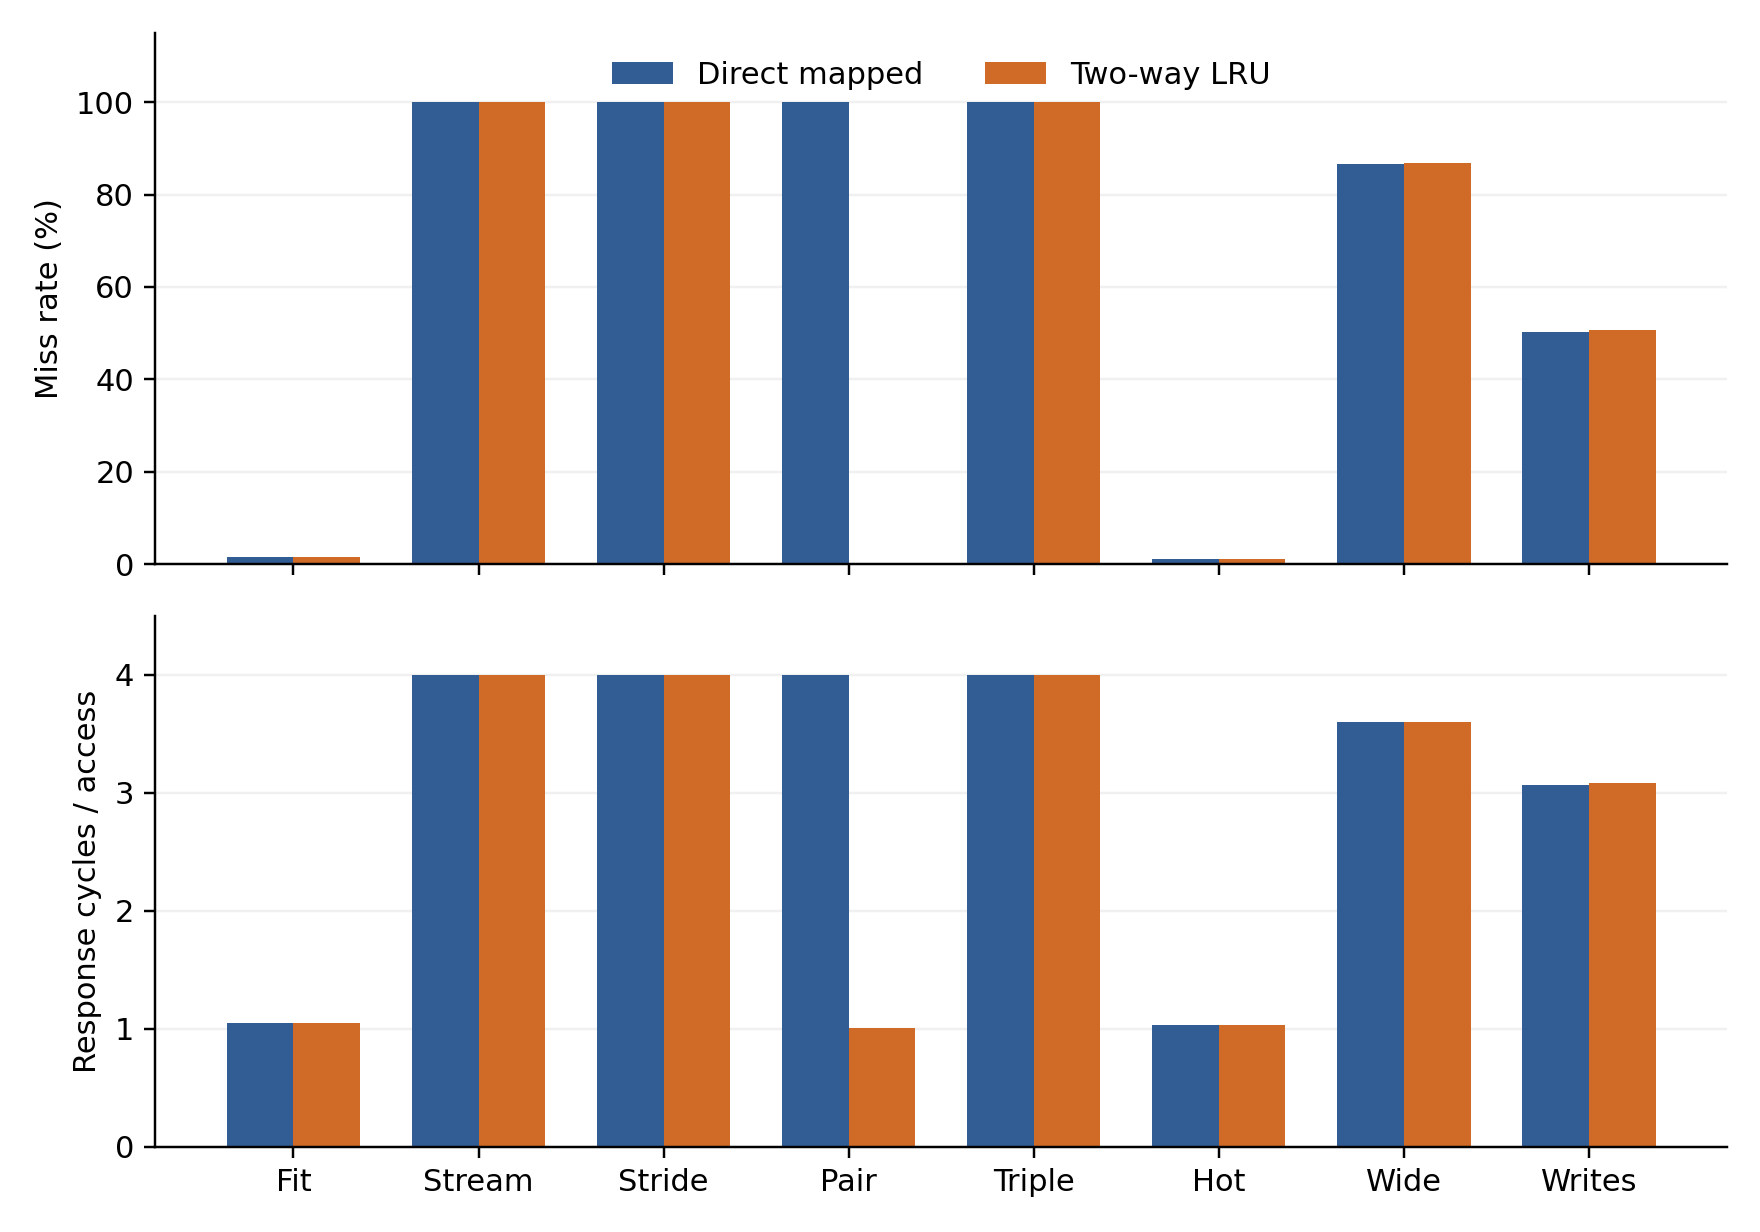
\includegraphics[width=0.84\textwidth]{../results/comparison.png}
\caption{Measured miss rates and response latency for the equal-data-capacity
organizations. Fit, stream, stride, pair, triple, hot, wide, and writes follow
Table~\ref{tab:workloads}. Each bar summarizes 2,048 accesses.}
\label{fig:results}
\end{figure*}

\subsection{Associativity and Mapping}
The conflict pair produces the largest improvement. Both word indices zero
and thirty-two map to the same direct-mapped set. Alternation replaces the
other line each time, causing 2,048 misses. They also share a two-way set,
but both can remain resident. After two compulsory misses, 2,046 accesses hit.
The miss rate is 100\% for direct mapping and approximately 0.098\% for two
ways. Average response latency falls from 4.000 to 1.003 cycles under the
chosen memory model.

The conflict triple needs three lines in a single two-way set. Its cyclic
reuse continually displaces the next required line, so both organizations
miss on every access. Stride 16 touches only sixteen distinct words, yet
their mapping restricts them to one two-way set or two direct-mapped sets.
Both therefore thrash despite a working set smaller than total capacity.
These traces distinguish total capacity from per-set occupancy.

The fit trace has 32 compulsory misses and then hits in both designs.
The hot trace has 24 compulsory misses and subsequent hits. The streaming
working set contains 256 words; a sequential pass evicts lines before
reuse, so both designs miss on all 2,048 accesses.

\subsection{Random Access and Write Traffic}
For wide random access, direct mapping has 1,776 misses and two-way LRU has
1,777. Average response latency is approximately 3.602 and 3.603 cycles,
respectively. The difference is one miss in a single seeded synthetic trace,
which offers little basis for a general ranking.

In the mixed-write trace, direct mapping records 1,028 misses and 384
write-backs; two-way LRU records 1,040 misses and 383 write-backs.
Equation~\ref{eq:latency} gives 3.068 and 3.084 cycles per access.
The two-way cache saves one write-back but incurs twelve additional misses.
Thus its latency is slightly higher on this trace. Mapping changes together
with set count: greater associativity at fixed data capacity does not
guarantee fewer misses on every individual sequence.

\subsection{Cost and Limitations}
An analytical storage count gives $32(32+26+1+1)+16=1936$ bits for the two-way
cache and $32(32+25+1+1)=1888$ bits for the baseline. This includes data, tags,
valid and dirty bits, and two-way LRU state. It excludes controller registers
and combinational logic. Equal data capacity consequently differs from equal
total storage or implementation area.

The study uses synthetic traces, one random seed, word accesses, fixed memory
delay, and a single outstanding request. Sharing the controller reduces
timing differences between organizations but also shares its implementation
assumptions. The independent model validates observed data and traffic.
There is no cache flush, coherence protocol, byte-enable path, synthesis,
FPGA resource report, or measured maximum clock frequency in this evaluation.

\newpage
\balance
\section{Individual Contributions}
The Phase I repository contains contributions attributed to the team members.
Phase II extends those responsibilities as listed below. This delivery was
prepared with coding-assistant support and committed through Aaditya's account.
The responsibilities identify ownership for review and follow-up. Each member's
Phase II review record and individual follow-up commits remain pending at
the time of this delivery.
\begin{itemize}
\item Aaditya Yadav: memory behavior, trace verification, and result reproduction.
\item Gauri Mishra: shared controller, index parameterization, and integration.
\item Bhumi Rastogi: address mapping, arrays, and direct-mapped storage review.
\item Ansh Sharma: LRU decisions, conflict traces, and workload analysis.
\item Anugra: report, diagrams, references, and reproducibility review.
\end{itemize}
A repository review record is provided for members to add their actual work,
findings, and commit evidence. Each member should be able to explain both
the assigned area and the overall request-to-response flow.

\section{Conclusion}
The project delivers a working two-way LRU cache and an equal-data-capacity
baseline with reproducible RTL comparisons. The verification checks hit
classification, data values, memory traffic, and response timing.
Two-way associativity eliminates repeated misses for a conflicting pair,
while three competing blocks still exceed the set's capacity. Random and
mixed-write results show that this advantage depends on the trace.
Future evaluation can vary random seeds, replay application traces, add
flush support, and perform synthesis before making area or frequency claims.

\begin{thebibliography}{2}
\bibitem{hill}
M. D. Hill and A. J. Smith, \textquotedblleft Evaluating associativity in CPU
caches,\textquotedblright{} \emph{IEEE Trans. Comput.}, vol. 38, no. 12,
pp. 1612--1630, Dec. 1989, doi: 10.1109/12.40842.
\bibitem{mattson}
R. L. Mattson, J. Gecsei, D. R. Slutz, and I. L. Traiger,
\textquotedblleft Evaluation techniques for storage hierarchies,\textquotedblright{}
\emph{IBM Syst. J.}, vol. 9, no. 2, pp. 78--117, 1970,
doi: 10.1147/sj.92.0078.
\end{thebibliography}
\end{document}
